\begin{frame}
    \centering
    \begin{figure}
        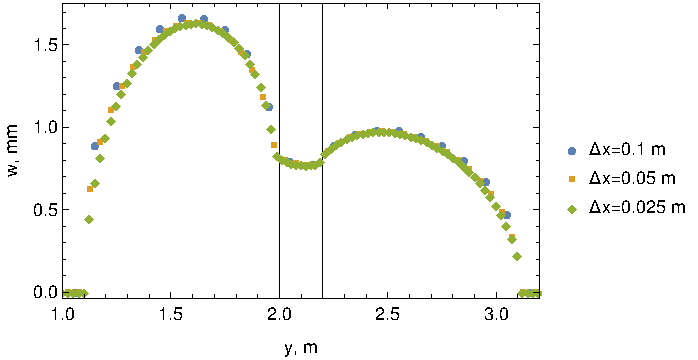
\includegraphics[width=0.7\textwidth]{static_accuracy.pdf}
        \caption{\footnotesize{Трехслойная среда, модуль Юнга и коэффициент Пуассона в слоях равны 1, 10, 2 GPa и 0.1, 0.4, 0.2 соответственно.}}
    \end{figure}

    \begin{tabular}{|c|c|c|}
        \hline
        $\Delta x, \text{м}$ & $E_{max}$ & $E_2$ \\
        \hline
        0.1                     & 0.129     & 0.059 \\
        \hline
        0.05                    & 0.096     & 0.028 \\
        \hline
        0.025 & --- & --- \\
        \hline
    \end{tabular}
\end{frame}

\begin{frame}
    \centering
    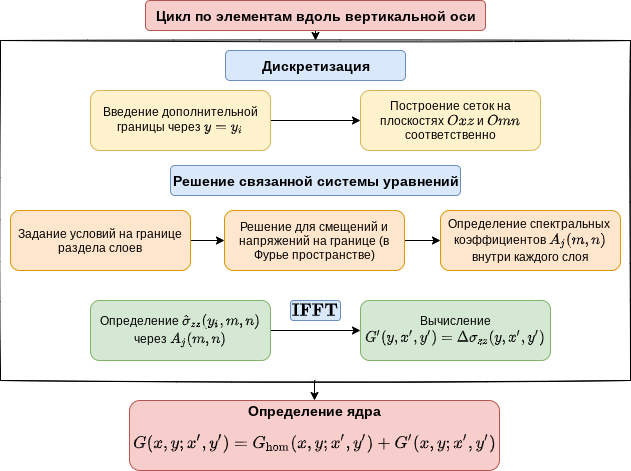
\includegraphics[width=0.9\textwidth]{scheme-layered.png}
\end{frame}

\begin{frame}
    \frametitle{Численная постановка}
    Дискретизация уравнений \eqref{eq:reynolds_equation} и \eqref{eq:elasticity_equation} осуществляется с помощью метода разрывных смещений
    \begin{equation}
        \label{eq:piecewiece_approximation}
        \begin{split}
            w(x,y,t) &= \sum\limits_{i,j} w_{i,j}(t) H_{i,j}(x,y), \\
            p(x,y,t) &= \sum\limits_{i,j} p_{i,j}(t) H_{i,j}(x,y), \\
        \end{split}
    \end{equation}
    где 
    \begin{equation}
        \label{eq:heaviside_function}
        H_{i,j}(x,y) = \left\{
            \begin{array}{ll}
                1, & (x,y) \in \mathcal{A}_{i,j}, \\
                0, & (x,y) \notin \mathcal{A}_{i,j}.
            \end{array}\right.
    \end{equation}
    Путём явного интегрирования по элементу уравнение упругости \eqref{eq:elasticity_equation} сводится к
    \begin{equation}
        \label{eq:discrete_elasticity}
        p_{i,j}(t) = {\sigma_h}_{i,j} + \sum\limits_{k,l} C_{i,j;k,l} w_{k,l}(t),
    \end{equation}
    где $C_{i,j;k,l}$ -- матрица упругости.
\end{frame}

\begin{frame}
    \frametitle{Дифференциальный оператор}
    \begin{equation*}
        \mathbb{A} = 
        \left[\begin{array}{cccccc}
            0                      & -\partial_x & -\partial_z & 0 & 0 & 0 \\
            -\frac{b}{a}\partial_x & 0           & 0 & 0 & \frac{b^2-a^2}{a}\partial_{xx} - \frac{f}{2}\partial_{zz} & \left( \frac{b^2-ab}{a} - \frac{f}{2} \right) \partial_{xz} \\
            -\frac{b}{a}\partial_z & 0           & 0 & 0 & \left( \frac{b^2-ab}{a} - \frac{f}{2} \right) \partial_{xz} & \frac{b^2-a^2}{a}\partial_{zz} - \frac{f}{2}\partial_{xx} \\
            \frac{1}{a}            & 0           & 0 & 0 & -\frac{b}{a}\partial_x & -\frac{b}{a}\partial_z \\
            0                      & \frac{2}{f} & 0 & -\partial_x & 0 & 0 \\
            0                      & 0           & \frac{2}{f} & -\partial_z & 0 & 0 
        \end{array}\right],
    \end{equation*}
    
    где используются константы
    \begin{align*}
        a   & = \lambda + 2G,                          & b   & = \lambda,                &     f & = 2G, \\
        l_2 & = \frac{\lambda + 3G}{\lambda + G},      & l_4 & = \frac{2G^2}{\lambda+G}, &   l_5 & = \frac{2G(\lambda + 2G)}{\lambda + G}, \\
        l_6 & = \frac{2G(2\lambda + 2G)}{\lambda + G}, & l_7 & = \frac{2\lambda G}{\lambda+G}
    \end{align*}
\end{frame}

\begin{frame}
    \frametitle{Обозначения}
    \begin{equation}
        \label{eq:FT_special_variables}
        \begin{split}
            \hat{u}_s & = -i \frac{(m\hat{u}_x + n\hat{u}_z)}{k}, \\
            \hat{u}_t & = -i \frac{(n\hat{u}_x - m\hat{u}_z)}{k}, \\
            \hat{\tau}_s & = -i \frac{(m\hat{\sigma}_{xy} + n\hat{\sigma}_{yz})}{k}, \\
            \hat{\tau}_t & = -i \frac{(n\hat{\sigma}_{xy} - m\hat{\sigma}_{yz})}{k}. \\
        \end{split} 
    \end{equation}

    \begin{equation}
        \begin{split}
        Z_s & = 
        \left[
        \begin{array}{cccc}
            -fe^{-ky} & (l_4-fky)e^{-ky} & fe^{ky} & (l_4+fky)e^{ky} \\
            -fe^{-ky} & (l_5-fky)e^{-ky} & -fe^{ky} & -(l_5+fky)e^{ky} \\
            e^{-ky} & kye^{-ky} & e^{ky} & kye^{ky} \\
            e^{-ky} & (ky-l_2)e^{-ky} & -e^{ky} & -(ky+l_2)e^{ky} \\
        \end{array}
        \right],
        \\
        Z_t & = 
        \left[
        \begin{array}{cc}
            -\frac{f}{2}e^{-ky} & \frac{f}{2}e^{ky} \\
            e^{-ky} & e^{ky}
        \end{array}
        \right].
        \end{split}
    \end{equation}
\end{frame}

\begin{frame}
    \frametitle{Условие скачка смещений и напряжений на границе раздела псевдослоя}
    \begin{equation*}
        \left[ \hat{T} \right] = 
        \left[ \begin{array}{c} 
            0 \\ \frac{\Delta u(b^2 - a^2)}{a} \\ \frac{\Delta ub}{a} \\ 0 \\ 0 \\ 0 
        \end{array} \right]
        +
        \frac{m^2}{m^2+n^2} \left[ \begin{array}{c} 
            0 \\ \Delta u(a-b) \\ 0 \\ 0 \\ 0 \\ 0 
        \end{array} \right]
        +
        \frac{mn}{m^2+n^2} \left[ \begin{array}{c} 
            0 \\ 0 \\ 0 \\ 0 \\ \Delta u(a-b) \\ 0 
        \end{array} \right].
    \end{equation*}
\end{frame}

\begin{frame}
    \frametitle{t-система связанных уравнений}
    Коэффициенты в t-системе \eqref{eq:coupled_t-system} имеют вид
    \begin{equation*}
        \begin{split}
            A^{i}_t &= \frac{2}{f^{i}}\text{cosech}(kd^{i}),\\
            B^{i}_t &= \frac{2}{f^{i+1}}\text{cosech}(kd^{i+1}),\\
            C^{i}_t &= -\frac{2}{f^{i+1}}\coth(kd^{i+1}) - \frac{2}{f^{i}}\coth(kd^{i}),\\
            D^{i}_t &= \Delta \hat{u}^{i}_{t} + \frac{2}{f^{i+1}}\coth(kd^{i+1})\Delta\hat{\tau}_{t}^{i} 
            - \frac{2}{f^{i}}\text{cosech}(kd^{i})\Delta\hat{\tau}_{t}^{i-1},
        \end{split}
    \end{equation*}
    \begin{equation*}
        \hat{u}^{i}_{t} = \frac{2}{f^{i}}\coth(kd^{i})\hat{\tau}^{i}_{t} - \frac{2}{f^{i}}\text{cosech}(kd^{i}) (\hat{\tau}^{i-1}_{t} + \Delta\hat{\tau}^{i-1}_{t}).
    \end{equation*}
\end{frame}

\begin{frame}
    \frametitle{s-система связанных уравнений}
    \begin{minipage}[t]{0.49\linewidth}
        \begin{equation*}
            \begin{split}
                \textbf{A}^{i} & = -R^{i}_{tb},\\
                \textbf{C}^{i} & = R^{i+1}_{bb}-R^{i}_{tt},
            \end{split}
        \end{equation*}
    \end{minipage}
    \hfill
    \begin{minipage}[t]{0.49\linewidth}
        \begin{equation*}
            \begin{split}
                \textbf{B}^{i} & = R^{i+1}_{bt},\\
                \textbf{D}^{i} & = \Delta u^{i}-R^{i+1}_{bb}\Delta p^{i}+R^{i}_{tb}\Delta p^{i-1},
            \end{split}
        \end{equation*}
    \end{minipage}
    \vspace{5mm}
    
    где используются следующие соотношения:
    \begin{equation*}
        \begin{split}
            R_{tt} & = \frac{1}{D} \left[\begin{array}{cc}
                - l_{5}(th + k \cdot d \cdot se^{2}) & - (l_{4}\cdot th^{2} + f\cdot k^{2} \cdot d^{2} \cdot se^{2})\\
                - (l_{4}\cdot th^{2} + f\cdot k^{2} \cdot d^{2} \cdot se^{2})  & - l_{5}(th - k \cdot d \cdot se^{2}) 
            \end{array}\right],\\
            R_{bb} & = \frac{1}{D} \left[\begin{array}{cc}
                l_{5}(th + k \cdot d \cdot se^{2}) & - (l_{4}\cdot th^{2} + f\cdot k^{2} \cdot d^{2} \cdot se^{2}) \\
                - (l_{4}\cdot th^{2} + f\cdot k^{2} \cdot d^{2} \cdot se^{2})  & l_{5}(th - k \cdot d \cdot se^{2})
            \end{array}\right],\\
            R_{bt} & = \frac{1}{D} \left[\begin{array}{cc}
                - (th + k \cdot d)\cdot se & - k \cdot d \cdot th \cdot se \\
                k \cdot d \cdot th \cdot se & - (th - k \cdot d)\cdot se 
            \end{array}\right],\\
            R_{tb} & = \frac{1}{D} \left[\begin{array}{cc}
                (th + k \cdot d)\cdot se & - k \cdot d \cdot th \cdot se \\
                k \cdot d \cdot th \cdot se & (th - k \cdot d)\cdot se  
            \end{array}\right].\\
        \end{split}
    \end{equation*}
\end{frame}


\begin{frame}
    \frametitle{Верификация метода путем сравнения с известными литературными данными}

    \begin{minipage}[t]{0.4\linewidth}
        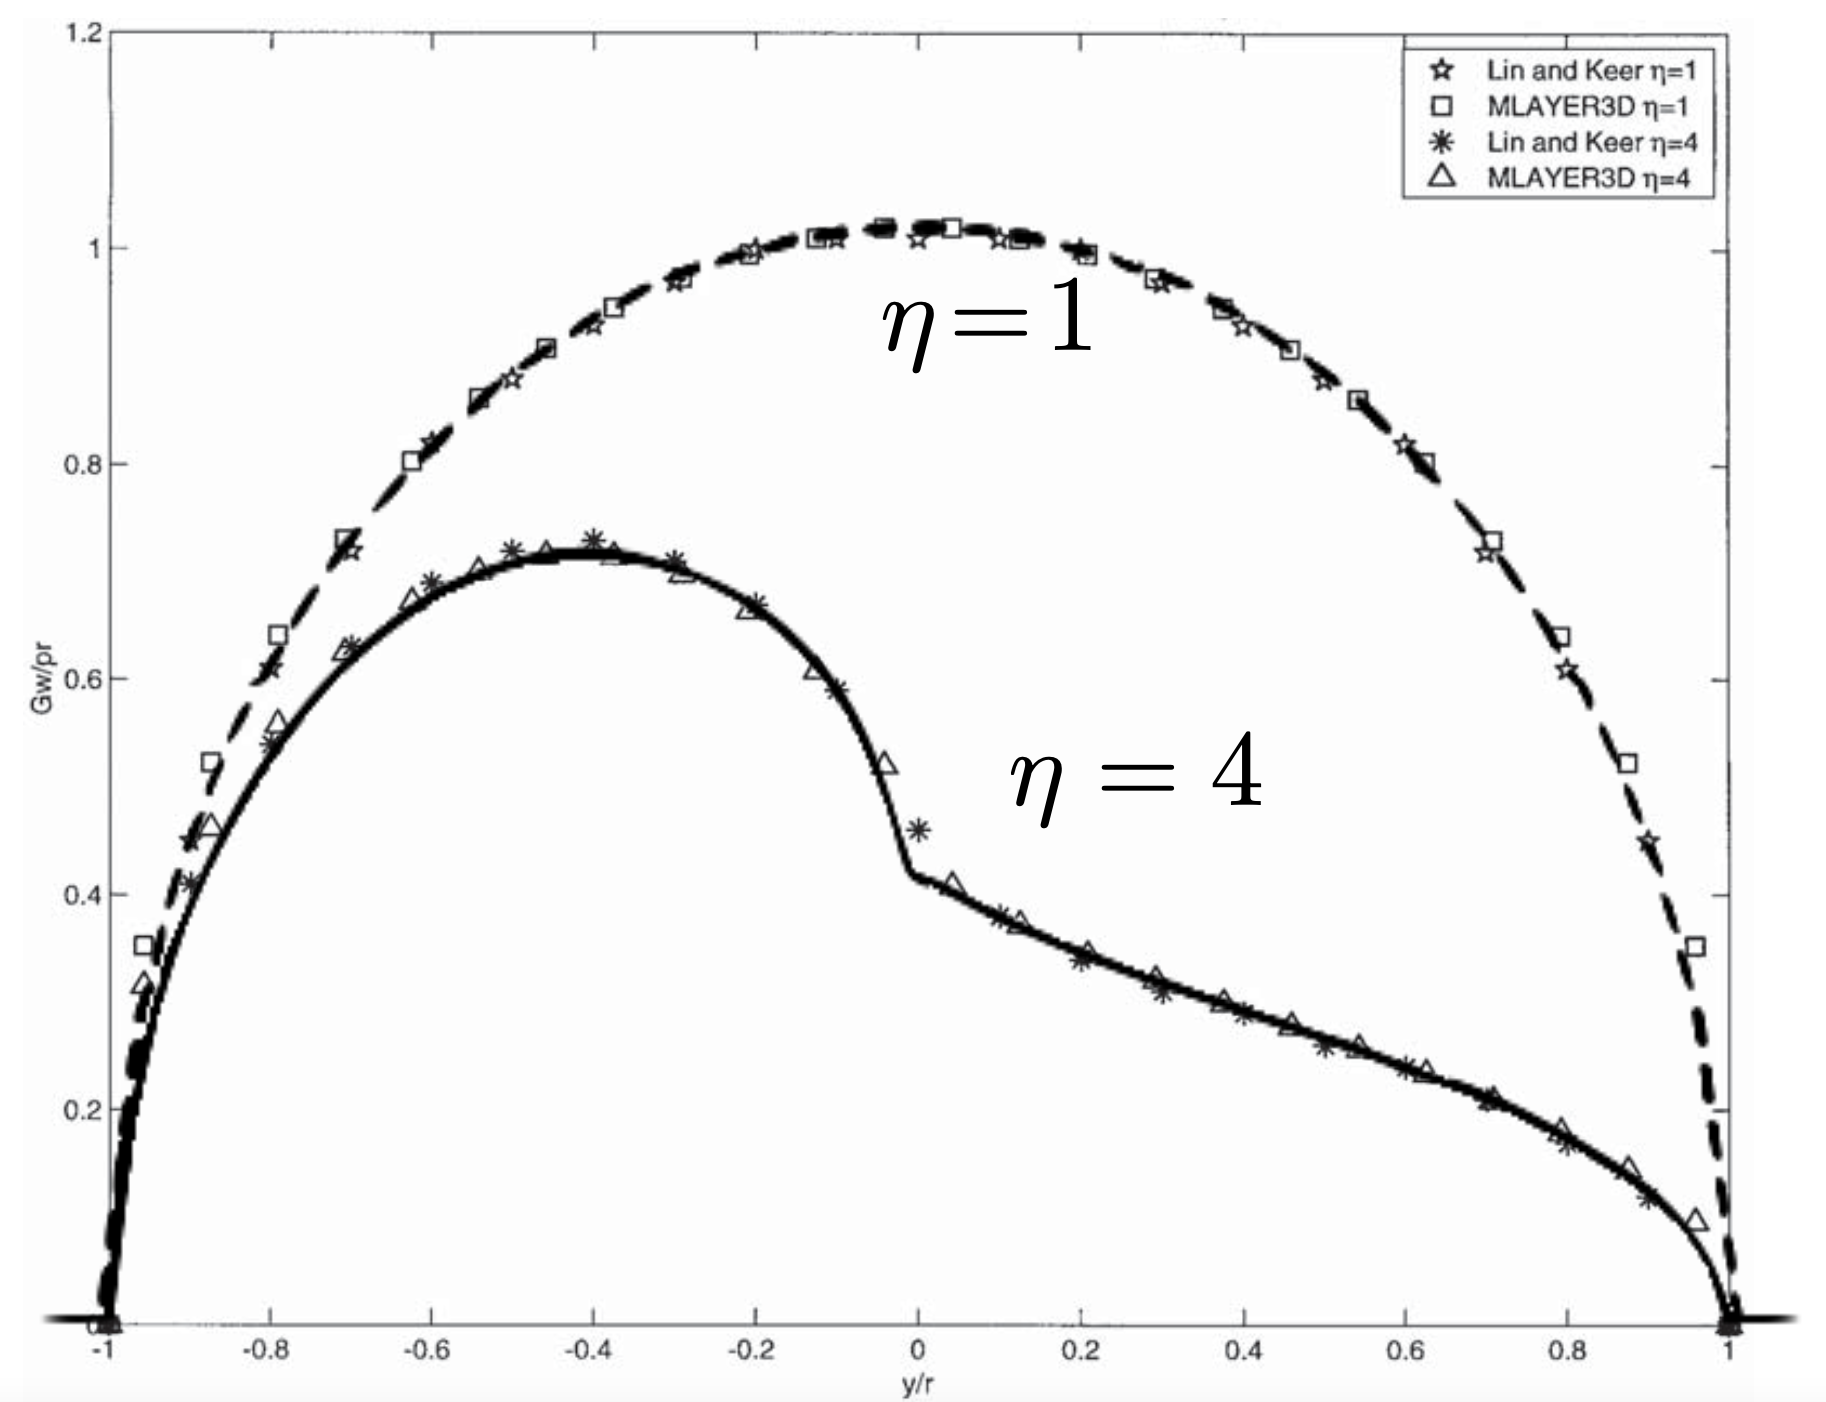
\includegraphics[width=\linewidth]{peirce-2layer.png}
    \end{minipage}
    \hfill
    \begin{minipage}[t]{0.57\linewidth}
        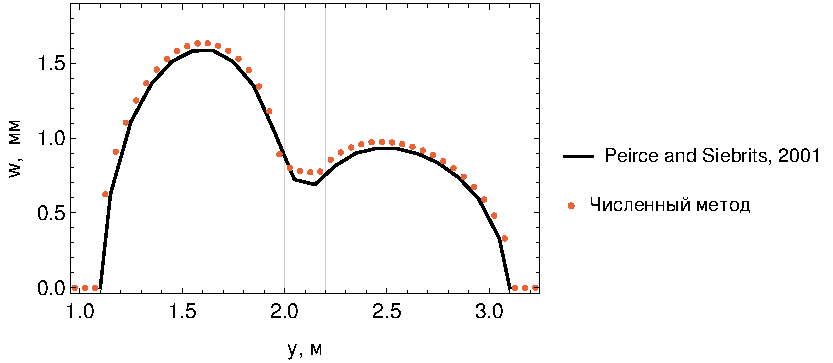
\includegraphics[width=\linewidth]{peirce-thin-layer.pdf}
    \end{minipage}
\end{frame}

